\section{Questionário}

\let\oldsubsection\thesubsection%
\renewcommand{\thesubsection}{\thesection.\alph{subsection}}

\subsection{O que é e para que serve o \textit{state array}?}

O \textit{state array} do \Keccak é uma representação do estado do algoritmo e
uma matriz de três dimensões, de tamanho $5 \times 5 \times w$, onde $w$ é o
comprimento do bloco a ser cifrado. Na maioria das linguagens de programação,
é uma estrutura muito simples de ser representada, mas tem um uso bastante
complexo no \Keccak.

As partes bidimensionais dessa matriz são chamadas de \textit{plane} (plano),
\textit{slice} (fatia) e \textit{sheet} (folha), e as unidimensionais são
chamadas de \textit{row} (linha), \textit{column} (coluna) e \textit{lane}
(pista), conforme mostrado na figura~\ref{fig:statearray}. Um bit é indexado
por sua linha, coluna e pista.

\begin{figure}[ht]
    \centering
    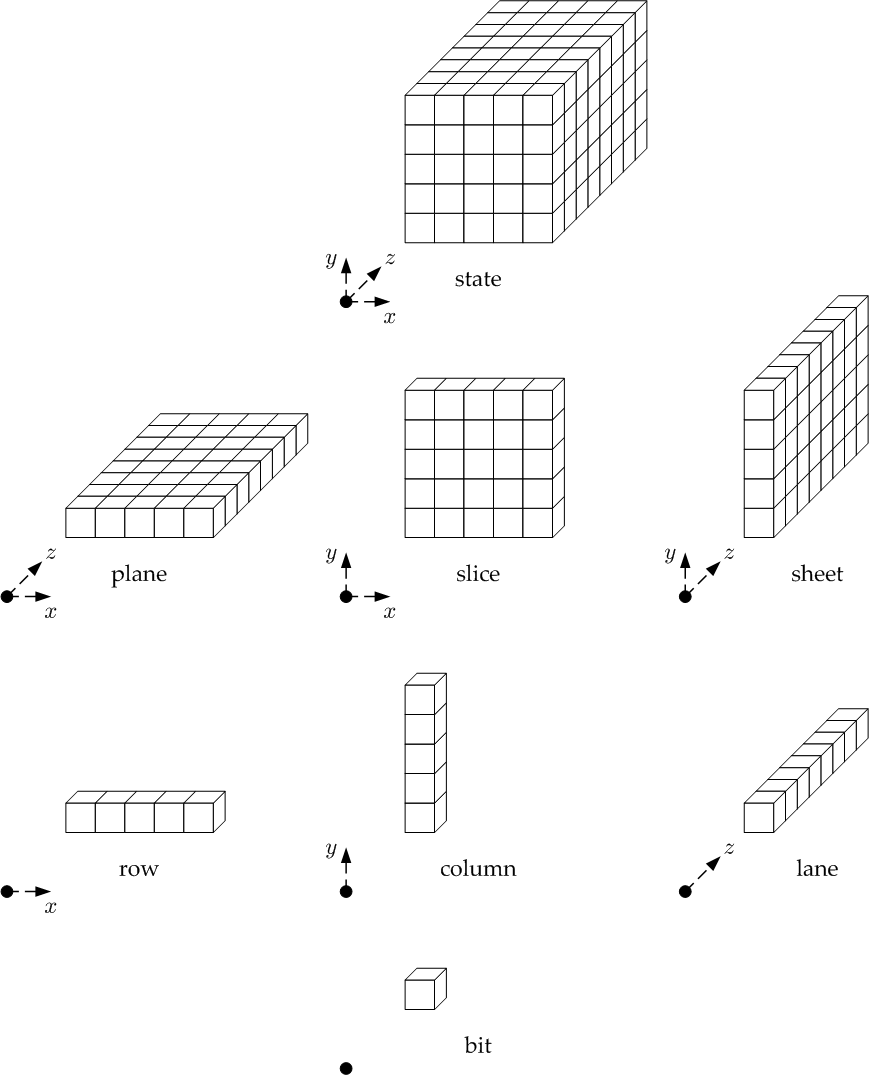
\includegraphics[width=0.7\textwidth]{images/statearray.png}
    \caption{Diagrama do \textit{state array}}
    \label{fig:statearray}
\end{figure}

O uso do \textit{state array} permite que as funções internas sejam definidas
em termos de posições nessa matriz de forma prática. O estado guarda valores
parciais do \textit{hash} e todas as funções internas recebem como parâmetro
o estado atual e retornam como saída o estado atualizado.

O primeiro valor do estado é gerado à partir da mensagem $S$ a ser cifrada, e o
resultado do \text{hash} é o estado após o último passo convertido novamente em
\textit{string}, passos estes que serão explicados nas próximas questões.

\subsection{Como é feita a conversão de \textit{strings} para
    \textit{state array}?}

Seja $S$ uma \textit{string} de $b$ \textit{bits} que representa o estado da
permutação \Keccak-$p[b, n_{r}]$. O \textit{state array} $A$ é definido da
seguinte forma no SHA-3, usando $b = 1600$ e $w = 64$:

Para toda tripla $(x, y, z)$ tal que $0 \leq x < 5$, $0 \leq y < 5$ e
$0 \leq z < w$,

\begin{center}
    $A[x, y, z] = S[w \cdot 5y + w \cdot x + z = S[w \cdot (5y+x) + z]$
\end{center}

Por exemplo, a posição $A[2, 1, 4]$ é obtida do \textit{bit}
$S[64 \cdot (5 \cdot 1 + 2) + 4] = S[772]$ da \textit{string} de entrada.

Usando essa fórmula, os \textit{bits} são mapeados sequencialmente por pista,
coluna e linha, ou seja, os primeiros 64 \textit{bits} serão mapeados na pista
da coluna 0 e linha 0, os próximos serão mapeados na pista da coluna 1 e linha
0, e assim sucessivamente.

\subsection{Como é feita a conversão de \textit{state array} para
    \textit{strings}?}

A conversão inversa, ou seja, de \textit{state array} para \textit{string}, é
feita de forma análoga, concatenando todas as pistas por coluna e então por
linha. Em passos, primeiro se concatenam os \textit{bits} de uma pista:

$Lane(i, j) = A[i, j, 0] \cdot A[i, j, 1] \cdot \ldots \cdot A[i, j, w-1]$

Por exemplo, para a linha 0 e coluna 0, e usando $w = 64$:

$Lane(0, 0) = A[0, 0, 0] \cdot A[0, 0, 1] \cdot \ldots \cdot A[0, 0, 63]$

$Lane(1, 0) = A[1, 0, 0] \cdot A[1, 0, 1] \cdot \ldots \cdot A[1, 0, 63]$

E assim sucessivamente para todas as pistas. Cada plano é a concatenação de
todas as pistas na sua coluna, indexadas por $0 \leq j < 5$:

$Plane(j) = Lane(0, j) \cdot Lane(1, j) \cdot \ldots \cdot Lane(4, j)$

\subsection{Explicar os cinco passos de mapeamento (\textit{step mappings})}

\subsection{Explicar a permutação Keccak-p[b,nr].}

\subsection{Descrever o \textit{framework} \textit{sponge construction}}

\subsection{Explique a família de funções esponja Keccak}

\subsection{Explique a especificação da função SHA-3}

\begin{enumerate}[label=\roman*.]
    \item Funções de \textit{hash} SHA-3
    \item Funções de saída extendida
\end{enumerate}

\subsection{Explique a construção da esponja}

\subsection{Apresente a análise de segurança}

\subsection{Exemplos}

\let\thesubsection\oldsubsection%
